\documentclass{beamer}
\usepackage{tikz}

\usetheme{Warsaw}
\title{Moogle}
\author{Noel Pérez Calvo}
\begin{document}

\begin{frame}
    \begin{figure}[h]
      \center
      
\includegraphics[width=11cm]{moogle.png}
      \caption{Buscador}
      \label{fig:logo}
    \end{figure}
  \end{frame} 

  \section{El buscador}
  \begin{frame}{¿Qué es Moogle?}
    Moogle es un buscador de archivos .txt, el cual mediante una consulta debe entregar un grupo de nombres de textos ordenados por relevancia(máximo 3) mostrando una pequeña porción de los mismos donde salgan elementos de la query. Para determinar esta relevancia se utiliza el calculo del TF-IDF, así como también la función coseno.  
  
  \end{frame}
  \section{Funcionamiento}
  \begin{frame}{Preprocesamiento}
    
    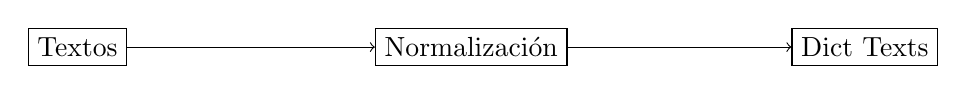
\begin{tikzpicture}
        \node[rectangle, draw] (A) at (2,0) {Textos};
        \node[rectangle, draw] (B) at (7,0) {Normalización};
        \draw[->] (A) -- (B);
        \node[rectangle, draw] (C) at (12,0) {Dict Texts};
        \draw[->] (B) -- (C);
      \end{tikzpicture}
    
      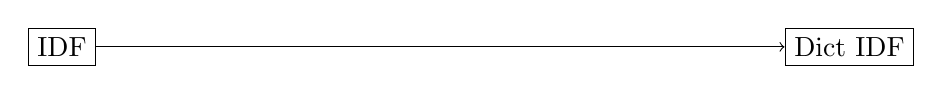
\begin{tikzpicture}
        \node[rectangle, draw] (A) at (0,-3) {IDF};
          \node[rectangle, draw] (B) at (10,-3) {Dict IDF};
          \draw[->] (A) -- (B);
        \end{tikzpicture} 
      
        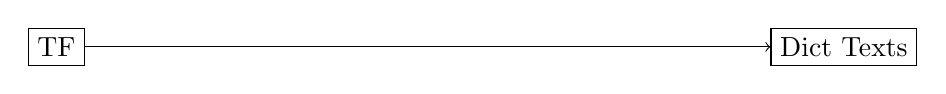
\begin{tikzpicture}
        \node[rectangle, draw] (A) at (0,-3) {TF};
          \node[rectangle, draw] (B) at (10,-3) {Dict Texts};
          \draw[->] (A) -- (B);
      \end{tikzpicture}
      Normalización: Eliminación de mayúsculas y caracteres no alfanuméricos
  
      Diccionario Texts: string,Diccionario de string,float
      \end{frame}  
  \begin{frame}{Preprocesamiento}
    \begin{tikzpicture}
    \node[rectangle, draw] (A) at (0,-3) {Dict Texts};
    \node[rectangle, draw] (B) at (0,-7) {Dict IDF};
    \node[rectangle, draw] (C) at (4,-5) {Cálculo TF-IDF};
    \node[rectangle, draw] (D) at (9,-5) {Dict Texts};
    \draw[->] (A) -- (C);
    \draw[->] (B) -- (C);
    \draw[->] (C) -- (D);
    \end{tikzpicture}
  \end{frame}

  \begin{frame}{Búsqueda}
    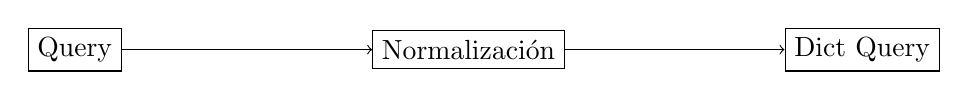
\begin{tikzpicture}
        \node[rectangle, draw] (A) at (2,0) {Query};
        \node[rectangle, draw] (B) at (7,0) {Normalización};
        \draw[->] (A) -- (B);
        \node[rectangle, draw] (C) at (12,0) {Dict Query};
        \draw[->] (B) -- (C);
      \end{tikzpicture}

      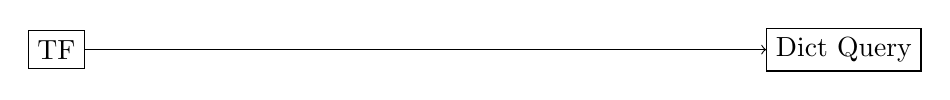
\begin{tikzpicture}
        \node[rectangle, draw] (A) at (0,-3) {TF};
          \node[rectangle, draw] (B) at (10,-3) {Dict Query};
          \draw[->] (A) -- (B);
      \end{tikzpicture}
      \begin{tikzpicture}
        \node[rectangle, draw] (A) at (0,-3) {Dict Query};
        \node[rectangle, draw] (B) at (0,-7) {Dict IDF};
        \node[rectangle, draw] (C) at (4,-5) {Cálculo TF-IDF};
        \node[rectangle, draw] (D) at (9,-5) {Dict Query};
        \draw[->] (A) -- (C);
        \draw[->] (B) -- (C);
        \draw[->] (C) -- (D);
      \end{tikzpicture}  
    
  \end{frame}

  \begin{frame}{Búsqueda}
    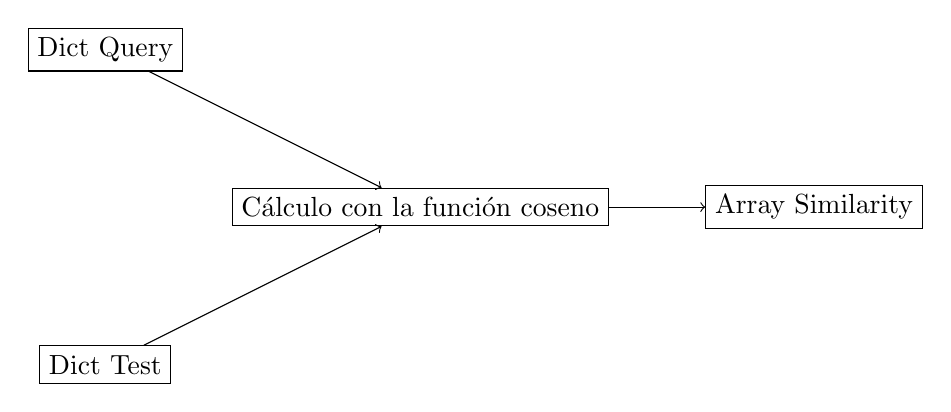
\begin{tikzpicture}
        \node[rectangle, draw] (A) at (0,-3) {Dict Query};
        \node[rectangle, draw] (B) at (0,-7) {Dict Test};
        \node[rectangle, draw] (C) at (4,-5) {Cálculo con la función coseno};
        \node[rectangle, draw] (D) at (9,-5) {Array Similarity};
        \draw[->] (A) -- (C);
        \draw[->] (B) -- (C);
        \draw[->] (C) -- (D);
    \end{tikzpicture}  

    
  \end{frame}
  
  
  \begin{frame}{Resultados}
    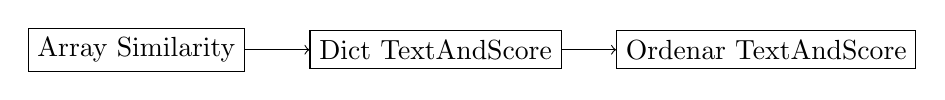
\begin{tikzpicture}
        \node[rectangle, draw] (A) at (3,0) {Array Similarity};
        \node[rectangle, draw] (B) at (6.8,0) {Dict TextAndScore};
        \draw[->] (A) -- (B);
        \node[rectangle, draw] (C) at (11,0) {Ordenar TextAndScore};
        \draw[->] (B) -- (C);
      \end{tikzpicture}

    

      A partir del Diccionario TextAndScore se toman los textos más importantes y se muestra el título y un pequeño Snippet
  \end{frame}
  \section{Muestra de los resultados}
  \begin{frame}{Si no coincide la búsqueda} 
    \begin{figure}[h]
      \center
      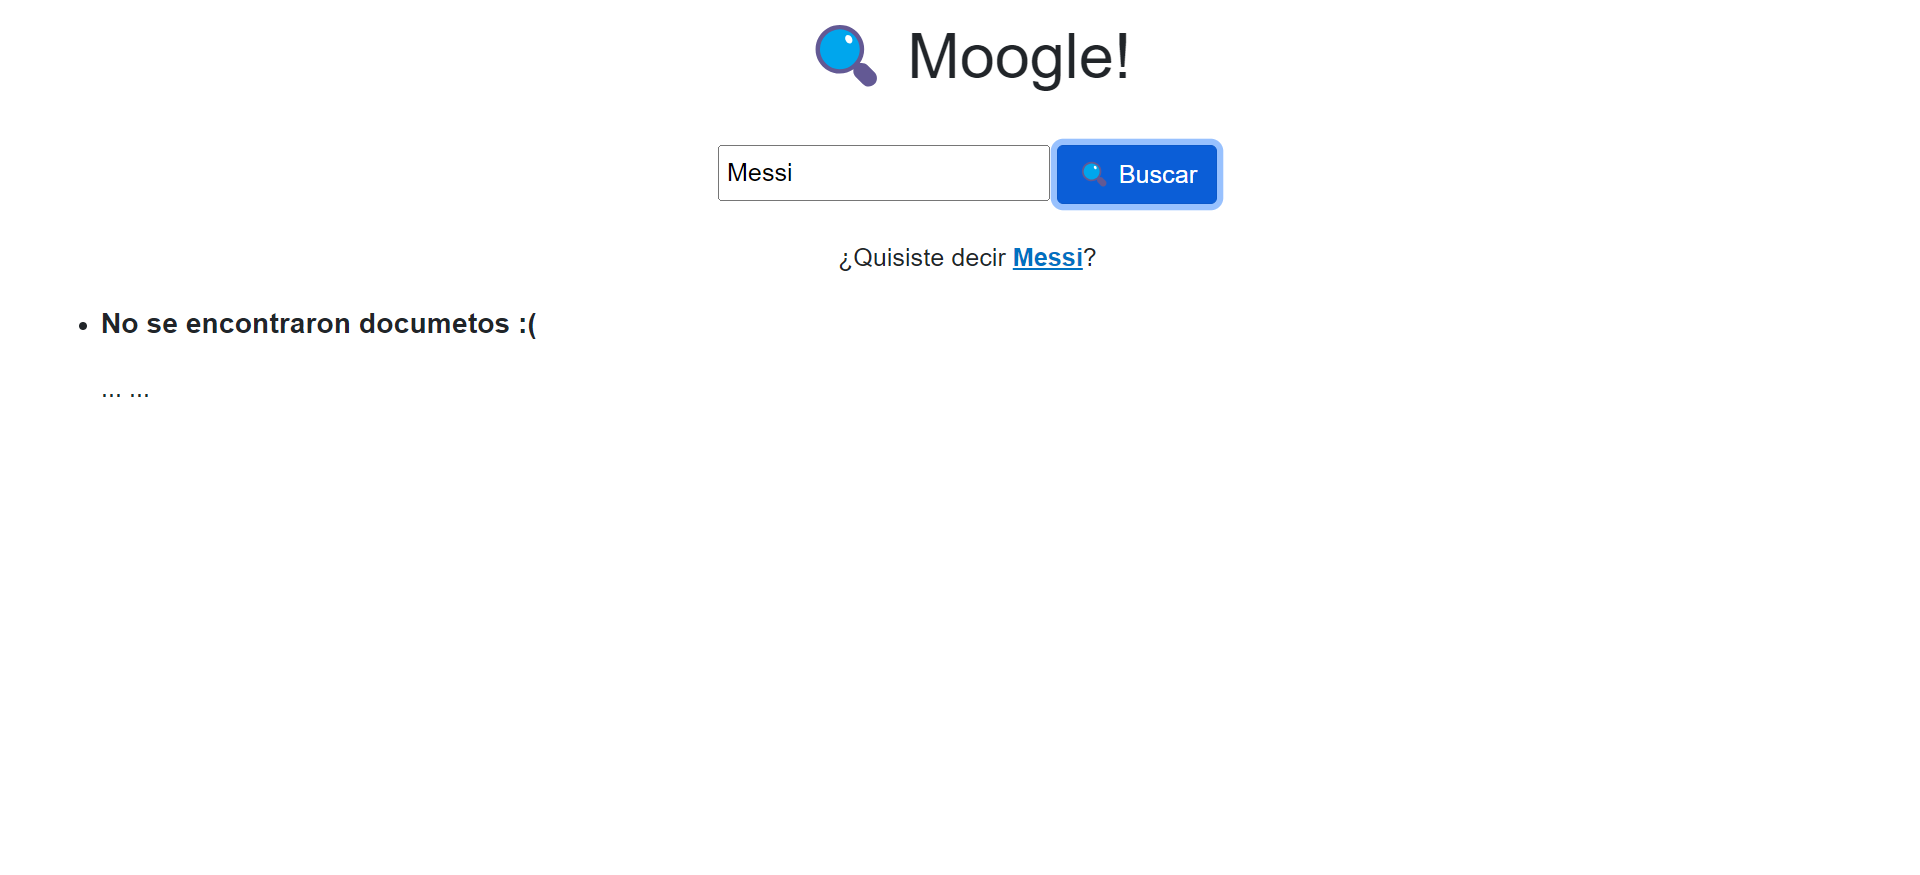
\includegraphics[width=11cm]{Ningun resultado.png}
      \caption{No hay coincidencias}
      \label{}
    \end{figure}
    
  \end{frame}
  \begin{frame}{Si coincide la búsqueda} 
    \begin{figure}[h]
      \center
      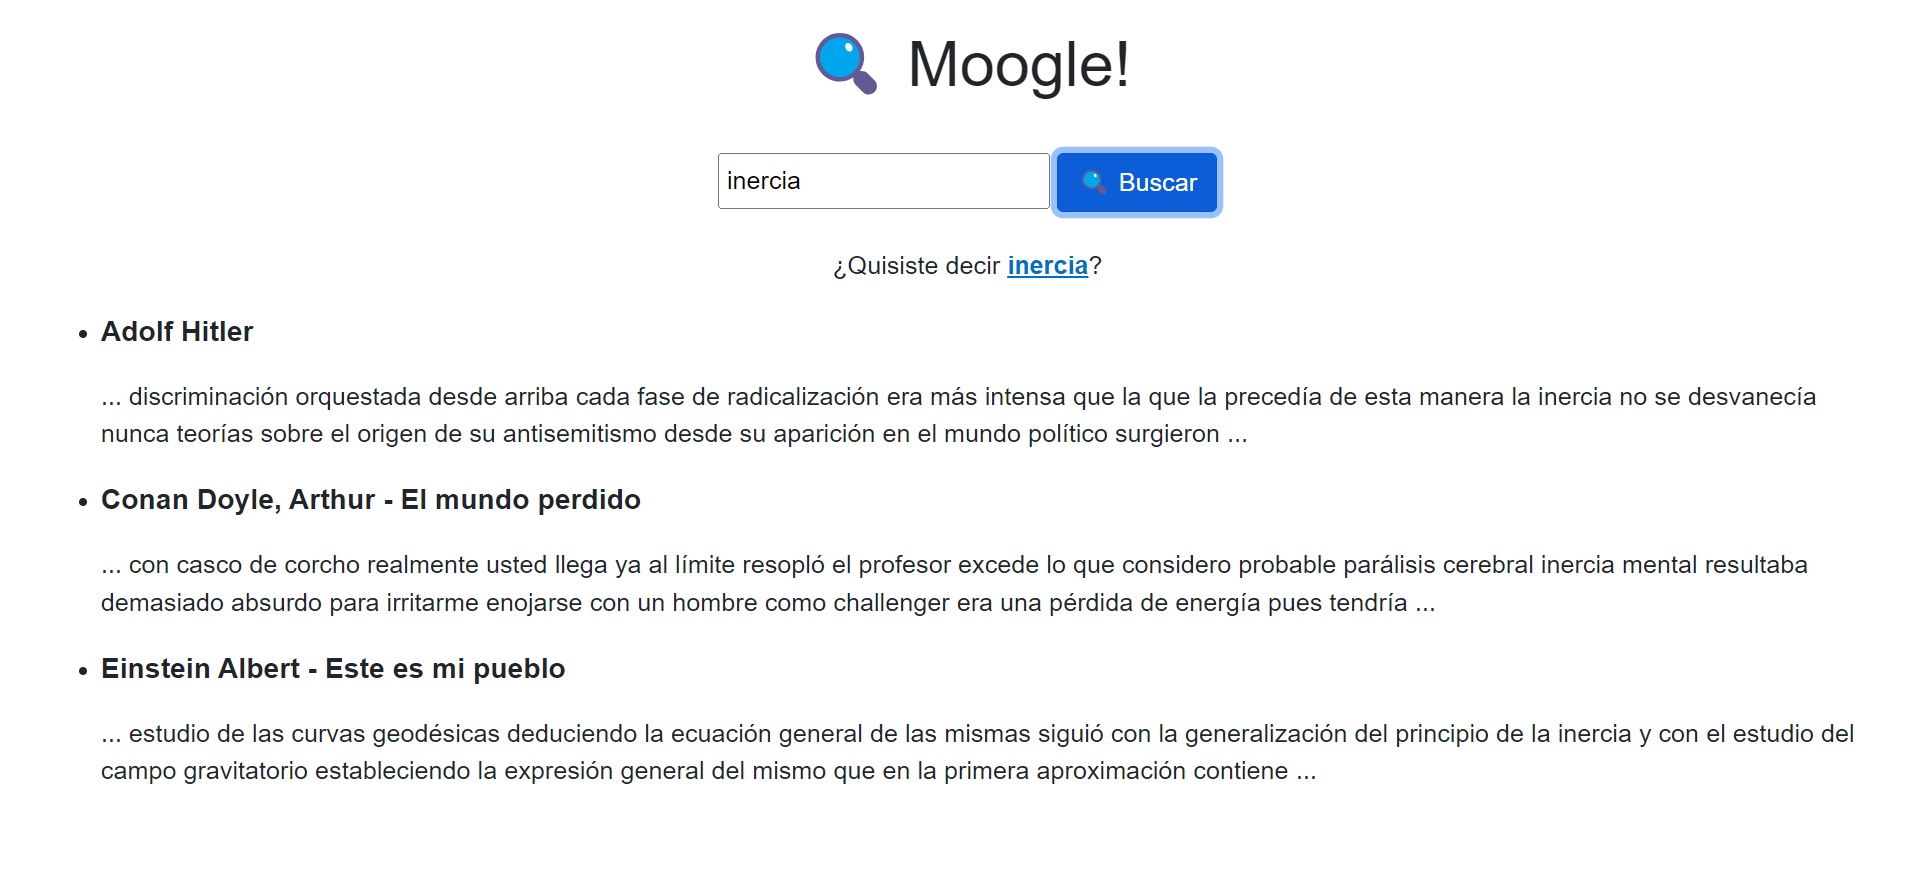
\includegraphics[width=11cm]{3 resultados.png}
      \caption{Las 3 coincidencias mas importantes}
      \label{}
    \end{figure}
    
  \end{frame}

  
  
  
  \section{Formulas Matemáticas}
  \begin{frame}{Función del ranking (Función Coseno)}
    \begin{equation}
        sim(d,q) = \frac{\vec{d_j}*\vec{q}}{{|\vec{d_j}|*|\vec{q}|}}
    \end{equation}
    \begin{equation}
        sim(d,q) = \frac{\sum_{i=1}^{n}w_i,_j*w_i,_q}{\sqrt{\sum_{i=1}^{n}w^2_i,_j}*\sqrt{\sum_{i=1}^{n}w^2_i,_q}}
       \end{equation}
\end{frame} 

\begin{frame}{Cálculo del peso en los documentos}
    \begin{equation}
        TF-IDF_i,_j = tf_i,_j * idf_i
    \end{equation}
    \begin{equation}
        tf_i,_j = \frac{freq_i,_j}{max_l freq_l,_j}
    \end{equation}
    \begin{equation}
        idf_i = \log \frac{N}{n_i}
    \end{equation}
    
\end{frame}



  
\end{document}

